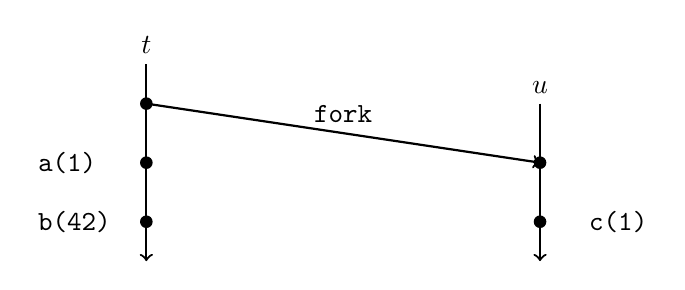
\begin{tikzpicture}
    \draw [->, thick] (4.5,-1) node[above] {$t$} -- (4.5,-3.5);
    \coordinate (a3) at (4.5,-1.5);
    \fill (a3) circle (0.08);
    \draw (3,-2.25) node[right] {\texttt{a(1)}};
    \coordinate (a4) at (4.5,-2.25);
    \fill (a4) circle (0.08);
    \draw (3,-3) node[right] {\texttt{b(42)}};
    \coordinate (a5) at (4.5,-3);
    \fill (a5) circle (0.08);

    \draw [->, thick] (9.5,-1.5) node[above] {$u$} -- (9.5,-3.5);
    \coordinate (b1) at (9.5,-2.25);
    \fill (b1) circle (0.08);
    \draw (10,-3) node[right] {\texttt{c(1)}};
    \coordinate (b2) at (9.5,-3);
    \fill (b2) circle (0.08);

    \draw[->, thick] (a3) to node[above] {\texttt{fork}} (b1);
\end{tikzpicture}
